\documentclass[11pt]{exam}
\usepackage{../commonheader}
\usepackage{graphicx}

\title{One-to-One and Onto Transformations}
\date{Week 7, Session 1}

\begin{document}
\maketitle

\section{Opening}
    
    \vspace{20px}
    \begin{questions}
        \item Let $T: \mathbb{R}^2 \rightarrow \mathbb{R^2}$ be a linear transformation induced by the matrix $A = \begin{bmatrix} 2 & 3 \\ 3 & 4 \end{bmatrix}$.
        How would we find $T$'s inverse? What would $T^{-1}$'s matrix be?
        \item Suppose $T[1,0]^T = [2,3]^T$ and $T[0,1]^T = [3,-1]^T$. What is the matrix associated with $T$?
    \end{questions}

\pagebreak
\section{One-to-One and Onto Transformations}
    
    \vspace{20px}
    Recall that a linear transformation maps vectors from $\mathbb{R}^n$ to $\mathbb{R}^m$, where the number of rows ($m$)
    and the number of columns ($n$) of the matrix of the transformation defines the dimensions of the pre and post-transformation spaces.

    Let's think conceptually:
    \begin{questions}
        \item Suppose $m > n$. Is it possible for \textit{every} vector in $\mathbb{R}^m$ to be the image of some vector in $\mathbb{R}^n$?
        \item Suppose $n > m$. Is it possible for \textit{every} vector in $\mathbb{R}^n$ to be the image of
        \textit{at most} one vector in $\mathbb{R}^n$?
    \end{questions}

    \vspace{20px}
    \subsection{One-to-One Transformations}
    A \textbf{one-to-one} transformation (or, an \textbf{injection}) is a transformation with the property that no vector in the post-transformation
    space is mapped to by more than one vector in the pre-transformation space.

    Transformations can be thought of as functions. If we consider an analagous function $f(x)$ like we're familiar with, a one-to-one function
    maps each $x$ value into a different $y$ value. In the graph below, $f(x) = x$ is one-to-one, but $f(x) = x^2$ isn't one-to-one, since it carries
    two $x$ values to $f(x) = 1$, for example.

    \begin{center}
        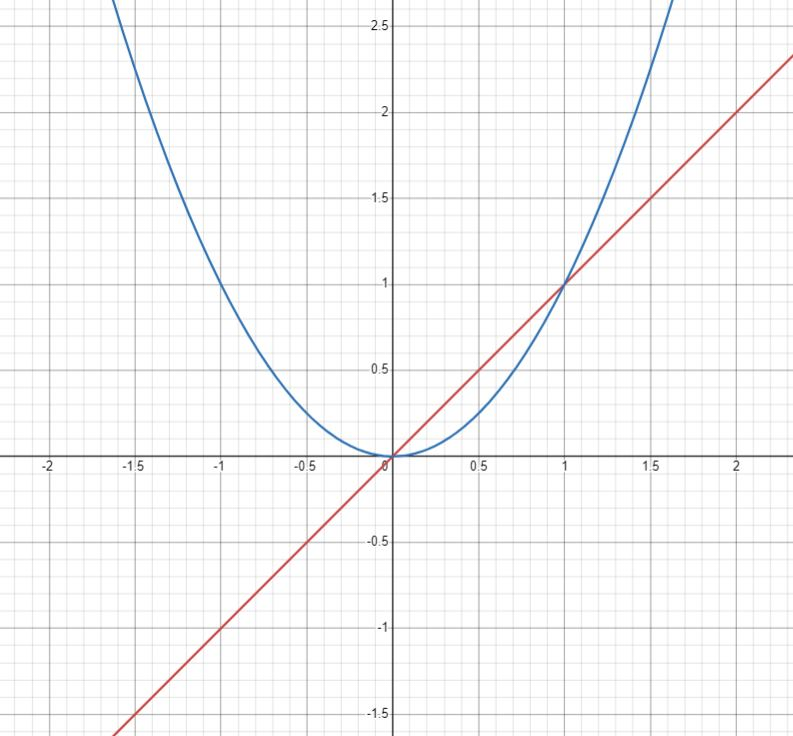
\includegraphics[width=0.5\textwidth]{one_to_one.JPG}
    \end{center}

    It turns out that we have a couple ways to immediately tell if a transformation is one-to-one:
    \begin{enumerate}
        \item If $A$ is the matrix of the transformation, $\text{rank}(A) = n$ (the dimension of the pre-transformation space)
        \item If the \text{only} vector which is mapped to $\vec{0}$ is the zero vector itself. This is the same as solving the homogeneous system
        $A \vec{x} = \vec{0}$ and verifying that it only has the trivial solution!
    \end{enumerate}

    \pagebreak
    \subsection{Onto Transformations}
    An \textbf{onto} transformation (or, a \textbf{surjection}) is a transformation with the property that every vector in the post-transformation
    space is mapped to by \textit{some} vector in the pre-transformation space.

    Using the same function analogy, an onto function is one where \textit{every} $y$ value is "touched" by the graph somewhere
    - even if it's more than once! $f(x) = x$ is onto, but $f(x) = \sqrt{x}$ is not (because negative values aren't mapped to by any $x$).
    \begin{center}
        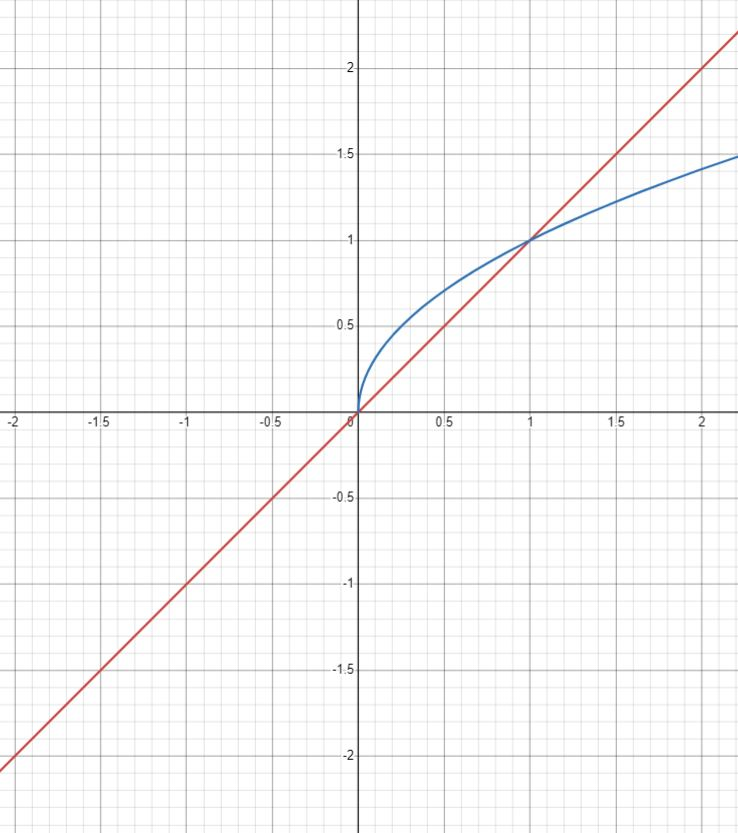
\includegraphics[width=0.5\textwidth]{onto.JPG}
    \end{center}

    Similarly, we can verify that a transformation is onto by checking if $\text{rank}(A) = m$ (the dimension of the post-transformation space)

    \pagebreak
    \section{Practice/Conceptual Questions}
    \begin{questions}
        \item Let $T: \mathbb{R}^3 \rightarrow \mathbb{R}^3$, and suppose $T$ is one-to-one. What is the rank of the transformation's
        corresponding matrix? Is $T$ onto?
        \item Let $T: \mathbb{R}^3 \rightarrow \mathbb{R}^2$, and suppose that $T$ is onto. Is it one-to-one?
        \item Let $T: \mathbb{R}^2 \rightarrow \mathbb{R}^3$. Is it possible for $T$ to be one-to-one? Onto?
        \item Let $T: \mathbb{R}^3 \rightarrow \mathbb{R}^3$, and suppose
        $T \begin{bmatrix} 1 \\ 0 \\ 0 \end{bmatrix} = T \begin{bmatrix} 2 \\ 0 \\ 0 \end{bmatrix} = \begin{bmatrix} 0 \\ 0 \\ 0 \end{bmatrix}$.
        Is $T$ one-to-one? Onto?
    \end{questions}

    


\end{document}